\chapter{细胞骨架动力学与细胞运动}\label{ch:b3:cytoskeleton-motility}

中性粒细胞在组织中追逐细菌，
以每分钟十微米的速度爬行，气味一变，几秒内便改变方向。
运动神经元细胞体中合成的神经递质囊泡，
沿轴突一直运到一米外的末梢，由一种马达蛋白牵引，
该马达蛋白每步八纳米，每秒走一百步，
持续两周。覆盖气管的\omterm{def:b3:cytoskeleton-motility:cilia}{纤毛}每秒摆动十二次，
形成协调的波，把一天吸入的灰尘送至喉部。这一切
都由三类蛋白丝完成，它们
在几秒内装配与拆解，并由每步水解一分子 ATP 的马达驱动。
细胞骨架并非固定框架意义上的骨架；
它是一组处于持续更替中的聚合物，其动力学
\emph{就是}形态、分裂与运动的机制。本章
讨论聚合物及其动力学、马达及限制它们的物理规律，
细胞的爬行，以及\omterm{def:b3:cytoskeleton-motility:cilia}{纤毛}与
鞭毛的摆动。

\section{三类聚合物}

\begin{definition}[肌动蛋白丝、微管与中间纤维]\label{def:b3:cytoskeleton-motility:filaments}
\index{肌动蛋白丝}\index{微管}\index{中间纤维}\index{极性!细丝}\index{中心体}
\emph{肌动蛋白丝}是由球状肌动蛋白组成的双链螺旋聚合物，
直径为 \qty{7}{nm}，每个亚基沿轴向长 \qty{2.7}{nm}，具有极性：\emph{带刺端}（正端）
生长比\emph{尖端}（负端）更快，
且每个亚基在掺入后携带的 ATP 会被水解。
\emph{微管}是中空管状结构，外径为 \qty{25}{nm}，
由十三条原纤维构成，每条原纤维由 $\alpha\beta$-微管蛋白二聚体组成，
（每个二聚体长 \qty{8}{nm}），同样具有极性，其\emph{正端}生长更快，
而\emph{负端}通常锚定在靠近细胞核的
\emph{中心体}上；$\beta$ 亚基在掺入后水解其
GTP。\emph{中间纤维}是绳状结构，
直径 \qty{10}{nm}，由卷曲螺旋蛋白构成（上皮中为角蛋白，
间充质中为波形蛋白，轴突中为神经丝蛋白，核纤层蛋白位于
核膜下方），无极性，不含核苷酸，稳定性远高于前两者——
它是承受张力的缆索，而非动态轨道。肌动蛋白主要位于
质膜下方和突起中；微管从
中心体辐射，充当长距离运输的轨道，并
构成纺锤体；中间纤维赋予细胞及其细胞核
机械韧性。
\end{definition}

\begin{omfigure}
\begin{tikzpicture}[every node/.style={font=\scriptsize}, >=stealth]
  % actin
  \begin{scope}
    \foreach \i in {0,...,11} { \fill[omThm!70] ({\i*0.4},{0.12*sin(\i*60)}) circle (0.17); }
    \node[below, align=center] at (2.2,-0.5) {肌动蛋白丝，\qty{7}{nm}\\双链螺旋，ATP-肌动蛋白 \\亚基沿轴向 \qty{2.7}{nm}};
    \node[left] at (-0.3,0) {$-$ 尖端}; \node[right] at (4.6,0) {带刺端 $+$};
  \end{scope}
  % microtubule
  \begin{scope}[xshift=7.2cm]
    \draw[thick, fill=omDef!25] (0,-0.55) rectangle (4.4,0.55);
    \foreach \y in {-0.35,-0.15,0.05,0.25} \draw[omDef] (0,\y) -- (4.4,\y);
    \foreach \x in {0.4,0.8,...,4.0} \draw[omDef] (\x,-0.55) -- (\x,0.55);
    \draw[thick] (4.4,0) ellipse (0.18 and 0.55); \draw[thick, fill=white] (4.4,0) ellipse (0.09 and 0.38);
    \node[below, align=center] at (2.2,-0.65) {微管，\qty{25}{nm}\\13 条原纤维，$\alpha\beta$-微管蛋白（GTP）\\二聚体长 \qty{8}{nm}};
    \node[left] at (-0.2,0) {$-$}; \node[right] at (4.7,0) {$+$};
  \end{scope}
  % intermediate filament
  \begin{scope}[yshift=-2.9cm, xshift=3.6cm]
    \foreach \dd in {-0.12,0,0.12} \draw[omMeth!70!black, thick] plot[domain=0:4.4, samples=60] (\x, {\dd + 0.1*sin(\x*200 + \dd*400)});
    \node[below, align=center] at (2.2,-0.4) {中间纤维，\qty{10}{nm}\\卷曲螺旋绳（角蛋白、波形蛋白、核纤层蛋白），无极性，无核苷酸};
  \end{scope}
\end{tikzpicture}

{\small 三种纤维按直径比例绘制。肌动蛋白与\omterm{def:b3:cytoskeleton-motility:filaments}{微管}蛋白
聚合物均具有极性，装配后水解核苷酸，这正是它们具有动态性的原因；
\omterm{def:b3:cytoskeleton-motility:filaments}{中间纤维}是无极性的绳状结构，
以耐久为特征。}
\end{omfigure}

\begin{omfigure}
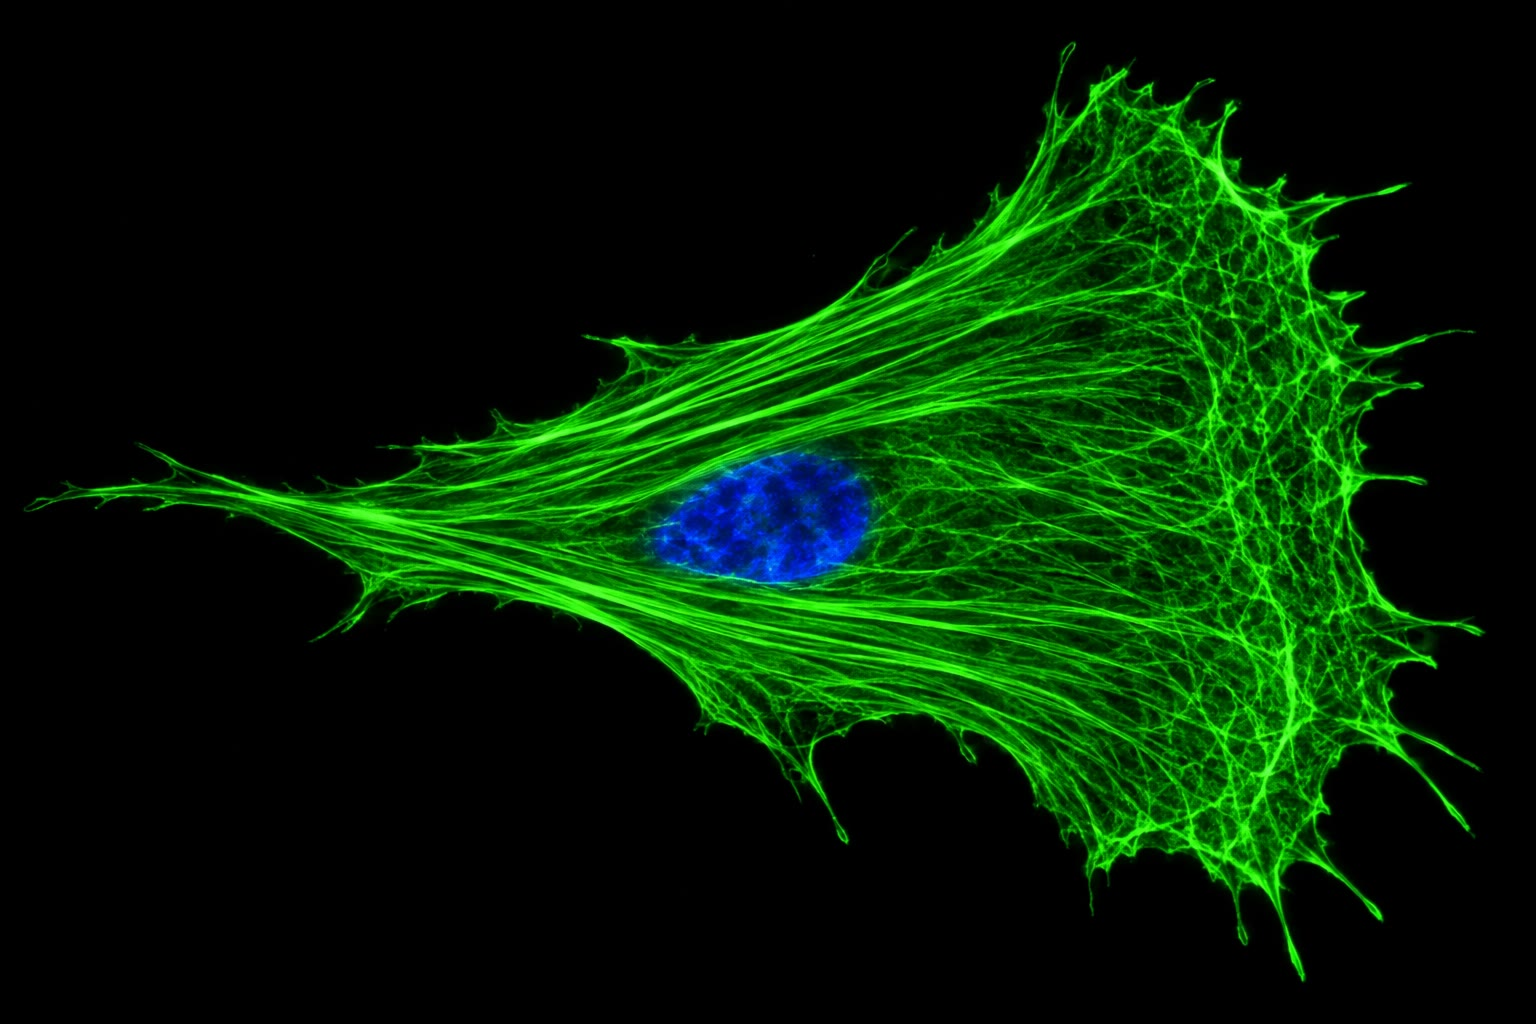
\includegraphics[width=0.54\linewidth]{images/book5/ai/b5-09-fibroblast-actin.jpg}\hspace{0.03\linewidth}
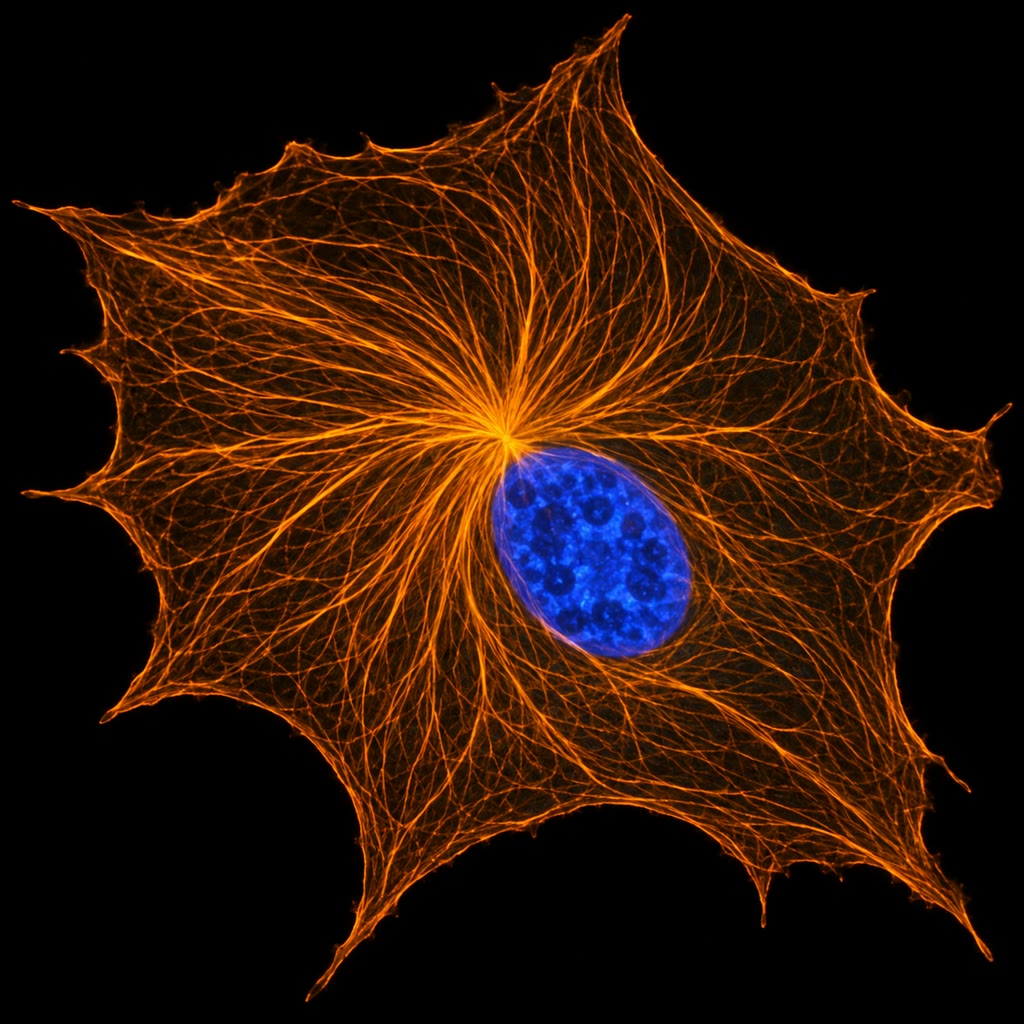
\includegraphics[width=0.36\linewidth]{images/book5/ai/b5-09-microtubules.jpg}

{\small 左：迁移中的成纤维细胞中的肌动蛋白（绿色）——应力纤维
贯穿细胞体，以及右侧宽阔前缘处的致密网络。右：\omterm{def:b3:cytoskeleton-motility:filaments}{微管}（橙色）
从\omterm{def:b3:cytoskeleton-motility:filaments}{中心体}辐射，\omterm{def:b3:cytoskeleton-motility:filaments}{中心体}位于细胞核（蓝色）旁，
一直延伸至细胞边缘。}
\end{omfigure}

\section{聚合物的动力学}

\begin{theorem}[临界浓度与踏车行为]\label{thm:b3:cytoskeleton-motility:treadmilling}
\index{临界浓度}\index{踏车行为}
设丝的某一端以速率 $k_{\mathrm{on}}C$ 添加亚基，其中
$C$ 为游离单体浓度，并以速率
$k_{\mathrm{off}}$ 失去亚基。若 $C$ 超过其\emph{\omterm{thm:b3:cytoskeleton-motility:treadmilling}{临界
浓度}} $C_{c} = k_{\mathrm{off}}/k_{\mathrm{on}}$ 时该端生长，低于它则缩短。
若两端的\omterm{thm:b3:cytoskeleton-motility:treadmilling}{临界浓度}不同，$C_{c}^{+}
< C_{c}^{-}$，则在丝既不伸长也不缩短的稳态下，
单体浓度为
\[
C_{\text{ss}} = \frac{k_{\mathrm{off}}^{+} + k_{\mathrm{off}}^{-}}
{k_{\mathrm{on}}^{+} + k_{\mathrm{on}}^{-}},
\qquad C_{c}^{+} < C_{\text{ss}} < C_{c}^{-},
\]
且正端生长、负端缩短，
两者速率均为 $J = k_{\mathrm{on}}^{+}C_{\text{ss}} - k_{\mathrm{off}}^{+} > 0$：亚基
由正端流向负端穿过丝体——\emph{\omterm{thm:b3:cytoskeleton-motility:treadmilling}{踏车行为}}
——每个亚基的流动需水解一分子核苷酸作为代价。
\end{theorem}
\begin{proof}
端点处的净速率为 $k_{\mathrm{on}}C - k_{\mathrm{off}}$，在
$C_{c}$ 处为零。长度不变要求两端净速率之和为零，
由此得到 $C_{\text{ss}}$；它位于两个\omterm{thm:b3:cytoskeleton-motility:treadmilling}{临界浓度}之间，
因为它是二者的加权平均（$C_{\text{ss}} =
(k_{\mathrm{on}}^{+}C_{c}^{+} + k_{\mathrm{on}}^{-}C_{c}^{-})/(k_{\mathrm{on}}^{+}
+ k_{\mathrm{on}}^{-})$）。高于 $C_{c}^{+}$ 时正端生长；
低于 $C_{c}^{-}$ 时负端缩短；通量即正端的净速率。
同一化学聚合物的两端具有相同的 $C_{c}$（即
相同的平衡常数），因此两端的差异要求亚基
在掺入后发生变化——即 ATP 或 GTP 的水解——
这一变化使两端不同，并为亚基的定向流动提供能量。
\end{proof}

\begin{example}[肌动蛋白在试管中]\label{ex:b3:cytoskeleton-motility:actin-numbers}
对于肌动蛋白-ATP，$k_{\mathrm{on}}^{+} = \qty{11.6}{\micro M^{-1}.s^{-1}}$，
$k_{\mathrm{off}}^{+} = \qty{1.4}{s^{-1}}$（$C_{c}^{+} = \qty{0.12}{\micro
M}$）；$k_{\mathrm{on}}^{-} = \qty{1.3}{\micro M^{-1}.s^{-1}}$，
$k_{\mathrm{off}}^{-} = \qty{0.8}{s^{-1}}$（$C_{c}^{-} = \qty{0.6}{\micro
M}$）。于是 $C_{\text{ss}} = 2.2/12.9 = \qty{0.17}{\micro M}$，$J =
11.6\times 0.17 - 1.4 = 0.6$ 个亚基每秒，即 \qty{1.6}{nm/s}，
难以察觉。在细胞中，细丝的踏车运动快约一百倍，
原因是 cofilin 切断并剥离尖端的旧 ADP-肌动蛋白，
profilin 将新鲜的 ATP-肌动蛋白装到带刺端上，
而封端蛋白决定哪些带刺端可以生长：
裸露的聚合物提供机制，调节因子提供速度。
\end{example}

\begin{omfigure}
\begin{tikzpicture}
\begin{axis}[
  width=0.7\linewidth, height=5.6cm,
  axis x line=bottom, axis y line=left,
  xmin=0, xmax=1.0, ymin=-1.6, ymax=4,
  xlabel={游离肌动蛋白 ($\unit{\micro M}$)}, ylabel={净速率（亚基/s）},
  xlabel style={font=\small, at={(axis description cs:0.5,-0.12)}, anchor=north},
  ylabel style={font=\small},
  tick label style={font=\small}, xtick={0,0.2,0.4,0.6,0.8,1.0}, ytick={-1,0,1,2,3,4},
  clip=false,
]
\addplot[thin, gray, domain=0:1.0, samples=2] {0};
\addplot[very thick, omThm, domain=0:0.46, samples=2] {11.6*x-1.4};
\addplot[very thick, omDef, domain=0:1.0, samples=2] {1.3*x-0.8};
\draw[dashed, gray] (axis cs:0.17,-1.6) -- (axis cs:0.17,4);
\node[font=\scriptsize, omThm, anchor=south east] at (axis cs:0.44,3.1) {带刺端};
\node[font=\scriptsize, omDef, anchor=north west] at (axis cs:0.62,-0.25) {尖端};
\node[font=\scriptsize, anchor=south west] at (axis cs:0.19,3.5) {$C_{\text{ss}}$};
\fill[omThm] (axis cs:0.12,0) circle (2pt); \node[font=\scriptsize, anchor=north east] at (axis cs:0.11,-0.05) {$C_{c}^{+}$};
\fill[omDef] (axis cs:0.6,0) circle (2pt); \node[font=\scriptsize, anchor=south west] at (axis cs:0.61,0.05) {$C_{c}^{-}$};
\end{axis}
\end{tikzpicture}

{\small \omterm{def:b3:cytoskeleton-motility:filaments}{肌动蛋白丝}每一端相对于游离单体的净生长速率，
取例中的速率常数。在两个\omterm{thm:b3:cytoskeleton-motility:treadmilling}{临界浓度}之间，
带刺端生长，尖端缩短；
在虚线处二者恰好抵消，细丝发生
踏车运动。}
\end{omfigure}

\begin{definition}[动态不稳定性]\label{def:b3:cytoskeleton-motility:instability}
\index{动态不稳定性}\index{GTP 帽}\index{灾变}
\omterm{def:b3:cytoskeleton-motility:filaments}{微管}的行为比踏车运动更为奇特。生长中的正端
带有由新加入二聚体构成的\emph{GTP 帽}；其后方的 GTP 被水解，
而倾向于弯曲构象的 GDP-微管蛋白被迫在晶格中保持直线排列，
处于应变之下。若帽丢失——
即末端暂停或生长减慢——应变的原纤丝向外卷开，
\omterm{def:b3:cytoskeleton-motility:filaments}{微管}以 \qty{300}{nm/s} 的速度缩短，约为其生长速率的二十倍：
这称为\emph{灾变}；当 GTP 二聚体落到末端并形成新帽时，
灾变结束，此即\emph{拯救}。
因此，在同一群体中，有些\omterm{def:b3:cytoskeleton-motility:filaments}{微管}在生长，而相邻的\omterm{def:b3:cytoskeleton-motility:filaments}{微管}却在崩溃：这就是
\emph{动态不稳定性}。它使细胞得以每隔几分钟用正端探查自身的体积，
并在\omterm{def:b3:cytoskeleton-motility:filaments}{中心体}移动或细胞分裂时重建整个\omterm{def:b3:cytoskeleton-motility:filaments}{微管}阵列。细胞通过
追踪正端的蛋白质来调控这一过程：这些蛋白质可以稳定（tau、MAP2）、
切断（katanin）或解聚（kinesin-13）\omterm{def:b3:cytoskeleton-motility:filaments}{微管}；
秋水仙碱和长春花生物碱阻止\omterm{def:b3:genomics:assembly}{组装}，紫杉醇阻止解聚，
这些药物均为有丝分裂纺锤体的毒物，
用于治疗癌症。
\end{definition}

\begin{proof}[证据]
米奇森和基施纳（1984）在体外观察了\omterm{def:b3:cytoskeleton-motility:filaments}{微管}群体，
它们从\omterm{def:b3:cytoskeleton-motility:filaments}{中心体}生长而来。将\omterm{def:b3:cytoskeleton-motility:filaments}{微管}蛋白稀释至\omterm{thm:b3:cytoskeleton-motility:treadmilling}{临界浓度}以下时，
他们预期所有\omterm{def:b3:cytoskeleton-motility:filaments}{微管}都会缓慢缩短；
结果\omterm{def:b3:cytoskeleton-motility:filaments}{微管}数量减少，而存活者却仍在生长——
有些迅速且完全地解聚，另一些则根本没有解聚。
随后以视频显微镜拍摄的单根\omterm{def:b3:cytoskeleton-motility:filaments}{微管}，
在稳定生长与快速缩短两个时期之间突然切换。
GTP 帽对两者都作出了解释：只有带帽的末端会生长，而帽的丢失
是一种罕见的、全或无的事件。
\end{proof}

\section{马达}

\begin{definition}[马达蛋白]\label{def:b3:cytoskeleton-motility:motors}
\index{肌球蛋白}\index{驱动蛋白}\index{动力蛋白}\index{持续性}
\emph{马达蛋白}将 ATP 水解的自由能转化为沿细丝的定向运动：
\emph{肌球蛋白}沿肌动蛋白运动（肌球蛋白 II 是肌肉和收缩性马达，
向带刺端运动；肌球蛋白 V 是双头囊泡运输体，
每步移动 \qty{36}{nm}），\emph{驱动蛋白}沿\omterm{def:b3:cytoskeleton-motility:filaments}{微管}向正端运动（驱动蛋白-1
每步移动 \qty{8}{nm}，即一个\omterm{def:b3:cytoskeleton-motility:filaments}{微管}蛋白二聚体，
每消耗一个 ATP 移动一步，以交替迈步的方式前进，速度约为
\qty{800}{nm/s}），而\emph{动力蛋白}向负端运动（胞质动力蛋白
借助其衔接蛋白 dynactin 将货物拖回细胞中心；\omterm{def:b3:cytoskeleton-motility:cilia}{轴丝动力蛋白}
使\omterm{def:b3:cytoskeleton-motility:cilia}{纤毛}弯曲）。若马达在脱离前能走许多步，则称其为
\emph{持续性的}：驱动蛋白-1 单独即可行走约一微米，即一百步；
而单个肌球蛋白 II 头部只完成一次冲程便松开，因此肌肉需要
数百个头部同时作用于同一根细丝。马达能够读取轨道的极性，
因此细胞的空间格局——正端位于周边，负端位于中心——
决定了每个马达将
货物运往何处。
\end{definition}

\begin{proof}[证据]
瓦勒、里斯和希茨（1985）发现了\omterm{def:b3:cytoskeleton-motility:motors}{驱动蛋白}，
它是鱿鱼轴浆中的一种蛋白质，能使乳胶珠沿\omterm{def:b3:cytoskeleton-motility:filaments}{微管}向正端滑动；
此后数年间，双头结构、各家族的运动方向，
以及其逆向伙伴\omterm{def:b3:cytoskeleton-motility:motors}{动力蛋白}，相继被厘清。斯沃博达、施密特、
施纳普和布洛克（1993）将携带单个\omterm{def:b3:cytoskeleton-motility:motors}{驱动蛋白}的小珠置于光阱中，
以纳米级\omterm{def:b3:structural-biology:methods}{分辨率}记录其位置：小珠以 \qty{8}{nm} 的离散步长前进，
低 ATP 浓度下每个 ATP 对应一步，
并在约 \qty{6}{pN} 的力作用下停止。
分子阶梯就这样，
被直接观察到了。
\end{proof}

\begin{omfigure}
\begin{tikzpicture}[every node/.style={font=\scriptsize}, >=stealth]
  % left: kinesin on a microtubule
  \begin{scope}
    \draw[thick, fill=omDef!25] (0,0) rectangle (5.4,0.5);
    \foreach \x in {0.4,0.8,...,5.2} \draw[omDef] (\x,0) -- (\x,0.5);
    \node[left] at (-0.1,0.25) {$-$}; \node[right] at (5.5,0.25) {$+$};
    % two heads, stalk, cargo
    \fill[omProp] (2.4,0.72) circle (0.2); \fill[omProp!60] (3.2,0.72) circle (0.2);
    \draw[thick, omProp!80!black] (2.6,0.85) -- (2.85,1.4) -- (3.05,0.85); \draw[thick, omProp!80!black] (2.85,1.4) -- (2.85,2.3);
    \draw[thick, fill=omExo!40] (2.85,2.7) circle (0.4); \node at (2.85,2.7) {货物};
    \draw[->, thick, omThm] (3.4,0.72) arc[start angle=180, end angle=0, radius=0.4] ; \node[right, omThm] at (3.85,1.15) {每 ATP \qty{8}{nm}};
    \node[below, align=center] at (2.7,-0.1) {驱动蛋白-1 手拉手地向正端行走；\\每秒约 $100$ 步，速度 \qty{0.8}{\micro m/s}};
  \end{scope}
  % right: optical trap staircase
  \begin{scope}[xshift=7.2cm, yshift=-0.6cm]
  \begin{axis}[
    width=5.6cm, height=4.4cm, axis lines=left,
    xmin=0, xmax=1.0, ymin=0, ymax=40,
    xlabel={时间 (s)}, ylabel={位置 (nm)},
    xlabel style={font=\scriptsize, at={(axis description cs:0.5,-0.12)}, anchor=north},
    ylabel style={font=\scriptsize},
    tick label style={font=\scriptsize}, xtick={0,0.5,1.0}, ytick={0,8,16,24,32},
  ]
  \addplot[very thick, omProp!80!black, const plot] coordinates {(0,0) (0.18,8) (0.31,16) (0.55,24) (0.71,32) (1.0,32)};
  \end{axis}
  \node[font=\scriptsize, align=center] at (2.8,3.6) {单个马达在光阱中，\\低 ATP：\qty{8}{nm} 步长};
  \end{scope}
\end{tikzpicture}

{\small \omterm{def:b3:cytoskeleton-motility:motors}{驱动蛋白}在其轨道上的行走，以及它在光阱中留下的足迹。
两个头交替运动，每一步使马达前进一个\omterm{def:b3:cytoskeleton-motility:filaments}{微管}蛋白二聚体，
即 \qty{8}{nm}；ATP 浓度低时，步与步之间
是等待下一个核苷酸的间隔，于是阶梯状的运动可以直接观察到。}
\end{omfigure}

\begin{proposition}[马达何以可能]\label{prop:b3:cytoskeleton-motility:physics}
\index{失速力}\index{热能}\index{扩散与运输}
细胞中一个 ATP 的水解释放约 \qty{50}{kJ/mol}，
即每个分子 $8\times 10^{-20}$ J。若马达每消耗一个 ATP 前进 $d$，
克服力 $F$ 做功 $Fd$，故其\emph{\omterm{prop:b3:cytoskeleton-motility:physics}{失速力}}
不超过 $F_{\max} = \Delta G/d$：对\omterm{def:b3:cytoskeleton-motility:motors}{驱动蛋白} \qty{8}{nm} 的步长，
上限为 \qty{10}{pN}；实测 \qty{6}{pN} 说明效率接近
\qty{60}{\%}，高于任何机器。\omterm{prop:b3:cytoskeleton-motility:physics}{热能} $k_{B}T =
4.1\times 10^{-21}$ J，即 \qty{4.1}{pN.nm}，只是 ATP 能量的二十分之一，
但它以布朗冲击的形式不断传给马达，
马达是一种能整流这些冲击的装置，让头部向前扩散，
并在落到合适位置时结合，使化学能
用于让这一步不可逆，而非用于推动。
在大细胞中，任何有意义的距离上，马达运输都优于扩散。
例如扩散系数为 $D = \qty{1}{\micro
m^2/s}$ 的囊泡，需时 $L^{2}/2D$ 才能游走 $L$ 的距离——游走一微米约需半秒，
但游走一米长的轴突则需 \num{16000} 年——
而马达以 \qty{1}{\micro m/s} 的速度，十二天即可走完这一米。
\end{proposition}
\admitted

\section{细胞如何爬行}

\begin{definition}[细胞迁移]\label{def:b3:cytoskeleton-motility:migration}
\index{片状伪足}\index{Arp2/3 复合体}\index{黏着斑}\index{整合素}\index{Rho 小 GTP 酶}
爬行细胞重复一个由四个步骤组成的循环。\emph{突出}：在
前缘处，肌动蛋白沿膜聚合成片，形成
\emph{片状伪足}，其分支网络由
\emph{Arp2/3 复合体}装配，它从已有细丝的侧面成核，
以 \qty{70}{\degree} 的分支角长出新细丝，封端蛋白限制每根细丝的生长，
丝切蛋白则使网络在后方数微米处被回收；
指状的\emph{丝状伪足}由成束细丝构成，向前探测。
\emph{黏附}：新的突出通过
\emph{整合素}连接基质，它是跨膜受体，外侧结合基质蛋白，
内侧借助接头蛋白结合肌动蛋白，聚集在
\emph{黏着斑}中。\emph{收缩}：\omterm{def:b3:cytoskeleton-motility:motors}{肌球蛋白} II 牵拉锚定于黏着斑的
应力纤维，拖动细胞主体向前。
\emph{回缩}：尾部的黏着斑松开，
尾部被拉回。该循环由三种小 GTP 酶协调，它们同属
\emph{Rho} 家族——Rac 驱动片状伪足，Cdc42 驱动丝状伪足，
Rho 驱动应力纤维与收缩——它们是
读取化学梯度方向（趋化性）的受体的靶标，这些受体
也可读取基质的硬度与图案。
\end{definition}

\begin{omfigure}
\begin{tikzpicture}[every node/.style={font=\scriptsize}, >=stealth]
  % substrate
  \draw[very thick, gray] (0,0) -- (12,0); \node[below right, gray] at (0,-0.05) {基质};
  % cell outline
  \draw[thick, omDef, fill=omDef!10] (1.0,0.05) .. controls (1.2,1.4) and (3.0,2.3) .. (5.0,2.2) .. controls (7.0,2.1) and (8.6,1.4) .. (9.8,0.6) .. controls (10.3,0.4) and (10.8,0.2) .. (11.2,0.05) -- cycle;
  % nucleus
  \draw[thick, fill=omDef!40] (4.6,1.1) ellipse (1.0 and 0.6); \node at (4.6,1.1) {细胞核};
  % lamellipodium: branched actin
  \foreach \p/\a in {(9.9,0.3)/20,(10.1,0.5)/-10,(10.3,0.25)/35,(10.6,0.45)/5,(10.4,0.7)/-25,(9.7,0.7)/15} { \draw[omThm, thick] \p -- ++(\a:0.55); \draw[omThm, thick] \p ++(\a:0.3) -- ++(\a+70:0.35); }
  \node[right, align=left, omThm] at (11.3,1.3) {1. 突出：\\Arp2/3 分支的肌动蛋白 \\推动细胞膜};
  \draw[->, thick, omThm] (11.3,0.3) -- (11.9,0.3);
  % focal adhesions
  \foreach \x in {9.3,7.6,2.4} \fill[omProp] (\x-0.25,0.03) rectangle (\x+0.25,0.18);
  \node[below, omProp, align=center] at (9.3,-0.45) {2. 黏附：整合素、\\黏着斑};
  % stress fibres and myosin
  \foreach \y in {0.45,0.75} \draw[omMeth!70!black, thick] (2.5,\y) -- (7.5,\y+0.1);
  \node[above, omMeth!70!black, align=center] at (7.8,2.3) {3. 收缩：肌球蛋白 II\\作用于应力纤维};
  \draw[->, thick, omMeth!70!black] (6.0,1.55) -- (6.8,1.55);
  % retraction at rear
  \draw[->, thick, gray] (0.8,0.9) -- (1.6,0.9); \node[above, align=center] at (1.4,2.35) {4. 回缩：\\后部黏着斑松开};
\end{tikzpicture}

{\small 爬行循环，从左至右为运动方向：分支肌动蛋白
聚合推动前缘向外伸出，\omterm{def:b3:cytoskeleton-motility:migration}{整合素}将其锚定，
\omterm{def:b3:cytoskeleton-motility:motors}{肌球蛋白}拉动细胞体向前，后部随之松开。}
\end{omfigure}

\begin{example}[李斯特菌的彗尾]\label{ex:b3:cytoskeleton-motility:listeria}
细菌 \emph{Listeria monocytogenes} 一旦进入细胞内，
在其表面展示一种单一的蛋白质 ActA，它募集宿主的
Arp2/3 复合体。肌动蛋白在细菌表面聚合，并
被留在身后形成尾巴；细菌被推动穿过细胞质，
速度可达 \qty{0.5}{\micro m/s}，并进入相邻细胞，全程从未
离开细胞溶胶。这一尾巴相当于翻转过来的\omterm{def:b3:cytoskeleton-motility:migration}{片状伪足}，
只用一种蛋白质，而细胞则需要数十种，这表明肌动蛋白
的聚合本身——不借助任何马达——即可产生
突出的力：每个亚基插入网络与膜之间，
当热涨落打开一道空隙时，使前缘棘齿式地
向前推进 \qty{2.7}{nm}。
\end{example}

\begin{method}[观察聚合物的更替]\label{met:b3:cytoskeleton-motility:frap}
\index{光漂白后荧光恢复}\index{斑点显微术}
测量活细胞中丝状结构系统的动力学：(1)
以低水平表达与荧光蛋白融合的亚基，使其
掺入内源聚合物；(2) 或用强激光脉冲
漂白一小块区域，并拍摄荧光随未漂白亚基交换
进入而恢复的过程（\emph{\omterm{met:b3:cytoskeleton-motility:frap}{光漂白后
荧光恢复}}，FRAP）——半衰期即
亚基的停留时间，永不恢复的部分即
不动池；或(3) 表达极少量标记亚基，使
聚合物呈稀疏的\emph{斑点}，并追踪它们：其
运动即踏车流动，其出现与消失即
\omterm{def:b3:genomics:assembly}{组装}与拆卸。在\omterm{def:b3:cytoskeleton-motility:migration}{片状伪足}中，斑点
相对于底物以每分钟约一微米的速度向后流动，而
边缘向前推进：网络在前缘构建，并在其后
数微米处被消耗。
\end{method}

\section{纤毛、鞭毛与旋转马达}

\begin{definition}[纤毛与鞭毛]\label{def:b3:cytoskeleton-motility:cilia}
\index{纤毛}\index{轴丝}\index{轴丝动力蛋白}\index{初级纤毛}\index{鞭毛内运输}
真核生物的\emph{纤毛}或\emph{鞭毛}是一种被膜包裹的
延伸结构，以\emph{轴丝}为基础：九组二联\omterm{def:b3:cytoskeleton-motility:filaments}{微管}
环绕一对中央\omterm{def:b3:cytoskeleton-motility:filaments}{微管}排列，由连接蛋白与辐条固定，并
从基体（一种由中心粒转化而来的结构）上生长。\emph{轴丝\omterm{def:b3:cytoskeleton-motility:motors}{动力蛋白}}
附着于每组二联\omterm{def:b3:cytoskeleton-motility:filaments}{微管}上，沿相邻二联\omterm{def:b3:cytoskeleton-motility:filaments}{微管}向其
基部的负端行走；由于二联\omterm{def:b3:cytoskeleton-motility:filaments}{微管}彼此相连，它们无法
自由滑动，滑动便转化为弯曲，并
沿轴丝以波的形式传播，通过将活跃\omterm{def:b3:cytoskeleton-motility:motors}{动力蛋白}
从环的一侧切换到另一侧。纤毛长 \qtyrange{5}{10}{\micro m}
，每秒搏动 \numrange{10}{20} 次；精子鞭毛长
\qty{50}{\micro m}，呈波浪状摆动。纤毛的蛋白质
由驱动蛋白-2 从细胞体向上运送，再由动力蛋白-2 沿
二联\omterm{def:b3:cytoskeleton-motility:filaments}{微管}向下运回，即\emph{鞭毛内运输}，这也是不能运动的
\emph{初级纤毛}——大多数脊椎动物细胞上每个细胞仅有一根——
的构建方式；该纤毛是一种感觉天线，
承载对光（视杆外段）、气味、流动与发育信号的受体，
其缺陷会导致\emph{纤毛病}：
多囊肾、视网膜变性、肥胖、多指（趾）。
\end{definition}

\begin{omfigure}
\begin{tikzpicture}[every node/.style={font=\scriptsize}, >=stealth]
  % axoneme cross-section
  \begin{scope}
    \draw[thick, omDef!60] (0,0) circle (1.75);
    \foreach \i in {0,...,8} { \begin{scope}[rotate=\i*40] \draw[thick, fill=omDef!30] (0,1.3) circle (0.16); \draw[thick, fill=omDef!30] (0.27,1.22) circle (0.13); \draw[omProp, thick] (0.15,1.05) -- (0.05,0.5); \draw[omThm, thick] (0.4,1.28) -- (0.62,1.2); \end{scope} }
    \draw[thick, fill=omDef!30] (-0.15,0) circle (0.16); \draw[thick, fill=omDef!30] (0.15,0) circle (0.16);
    \node[right, align=left] at (2.0,1.2) {9 组二联微管}; \draw (1.9,1.2) -- (1.35,1.0);
    \node[right, align=left] at (2.0,0.4) {中央微管对}; \draw (1.9,0.4) -- (0.35,0.1);
    \node[right, align=left, omThm] at (2.0,-0.4) {每组二联微管上的 \\动力蛋白臂伸向下一组}; \draw[omThm] (1.9,-0.3) -- (1.0,-0.85);
    \node[right, align=left, omProp] at (2.0,-1.3) {辐条}; \draw[omProp] (1.9,-1.3) -- (0.4,-0.7);
    \node[below] at (0,-1.9) {轴丝横截面，直径 \qty{0.25}{\micro m}};
  \end{scope}
  % bending from sliding
  \begin{scope}[xshift=7.6cm]
    \draw[very thick, omDef] (0,-1.6) -- (0,1.6); \draw[very thick, omDef] (0.5,-1.6) -- (0.5,1.6);
    \draw[->, thick, omThm] (0.1,0.5) -- (0.4,0.5); \draw[->, thick, omThm] (0.1,-0.2) -- (0.4,-0.2);
    \node[below, align=center] at (0.25,-1.7) {一组二联微管上的 \\动力蛋白推动相邻者 \\向尖端滑动};
    \draw[->, thick] (1.5,0) -- (2.5,0);
    \draw[very thick, omDef] (3.6,-1.6) .. controls (3.6,-0.3) and (4.6,0.5) .. (4.4,1.6); \draw[very thick, omDef] (4.1,-1.6) .. controls (4.1,-0.3) and (5.1,0.5) .. (4.9,1.6);
    \node[below, align=center] at (4.3,-1.7) {基部相连并由连接蛋白固定，\\二联微管无法滑动：\\于是弯曲};
  \end{scope}
\end{tikzpicture}

{\small \omterm{def:b3:cytoskeleton-motility:cilia}{轴丝}横截面（左）：九组二联\omterm{def:b3:cytoskeleton-motility:filaments}{微管}环绕一对
中央\omterm{def:b3:cytoskeleton-motility:filaments}{微管}，并带有\omterm{def:b3:cytoskeleton-motility:motors}{动力蛋白}臂与辐条。右：\omterm{def:b3:cytoskeleton-motility:motors}{动力蛋白}
使一组二联\omterm{def:b3:cytoskeleton-motility:filaments}{微管}沿相邻者滑动，由于二联\omterm{def:b3:cytoskeleton-motility:filaments}{微管}被系住，
滑动便转化为沿\omterm{def:b3:cytoskeleton-motility:cilia}{纤毛}传播的弯曲。}
\end{omfigure}

\begin{omfigure}
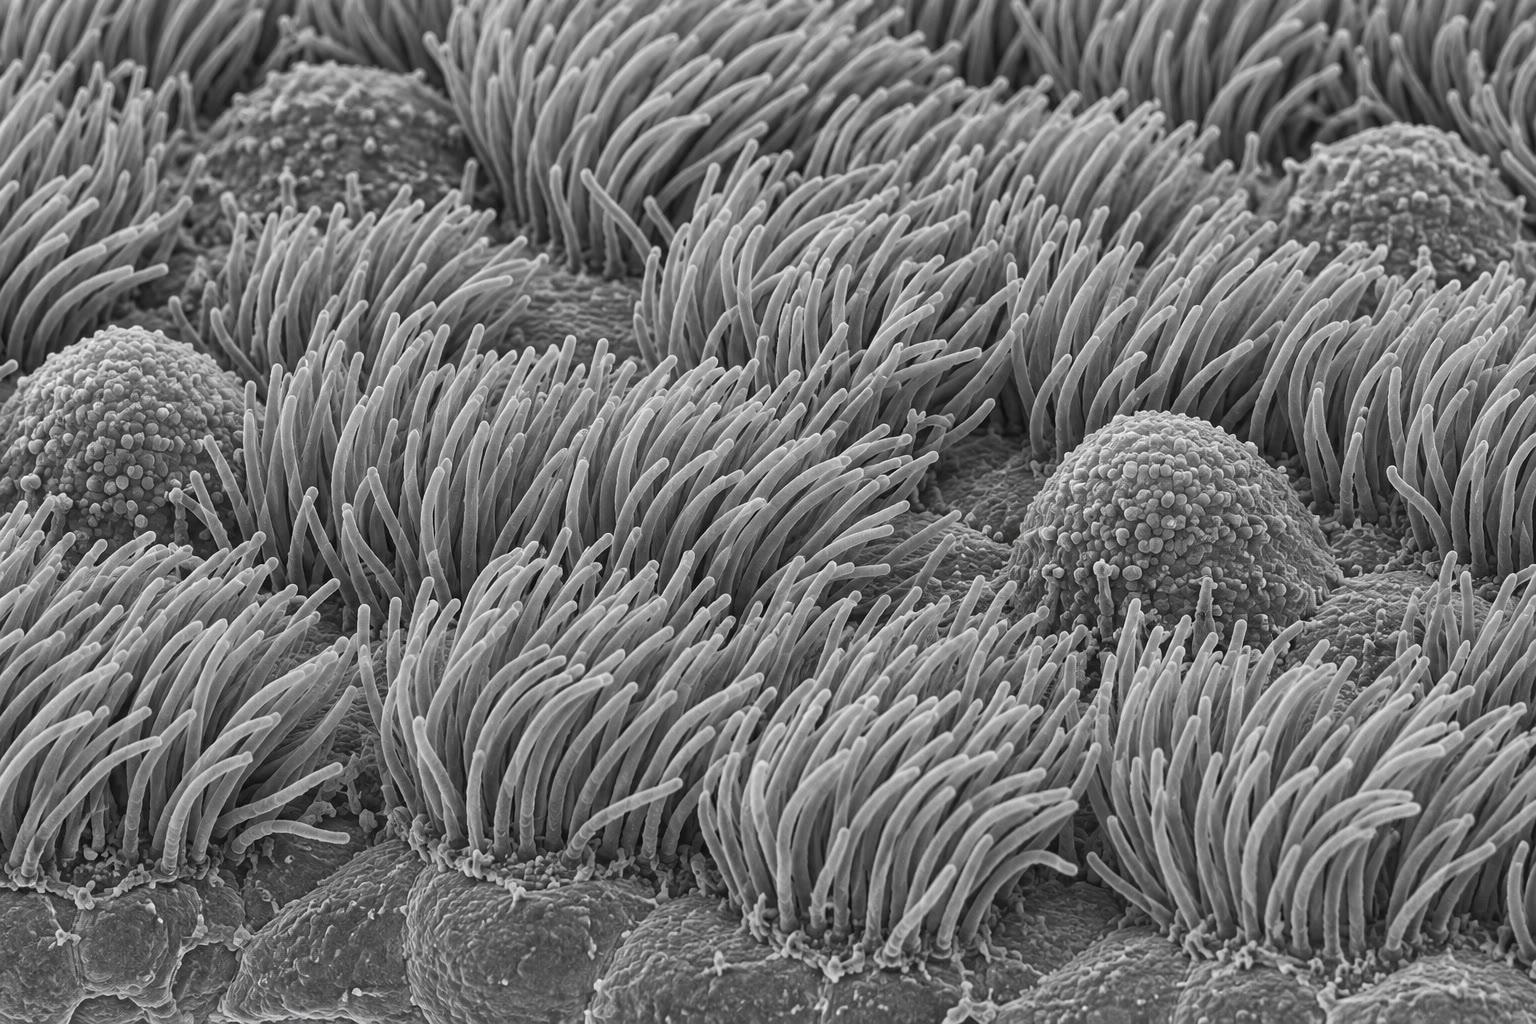
\includegraphics[width=0.54\linewidth]{images/book5/ai/b5-09-cilia-sem.jpg}\hspace{0.03\linewidth}
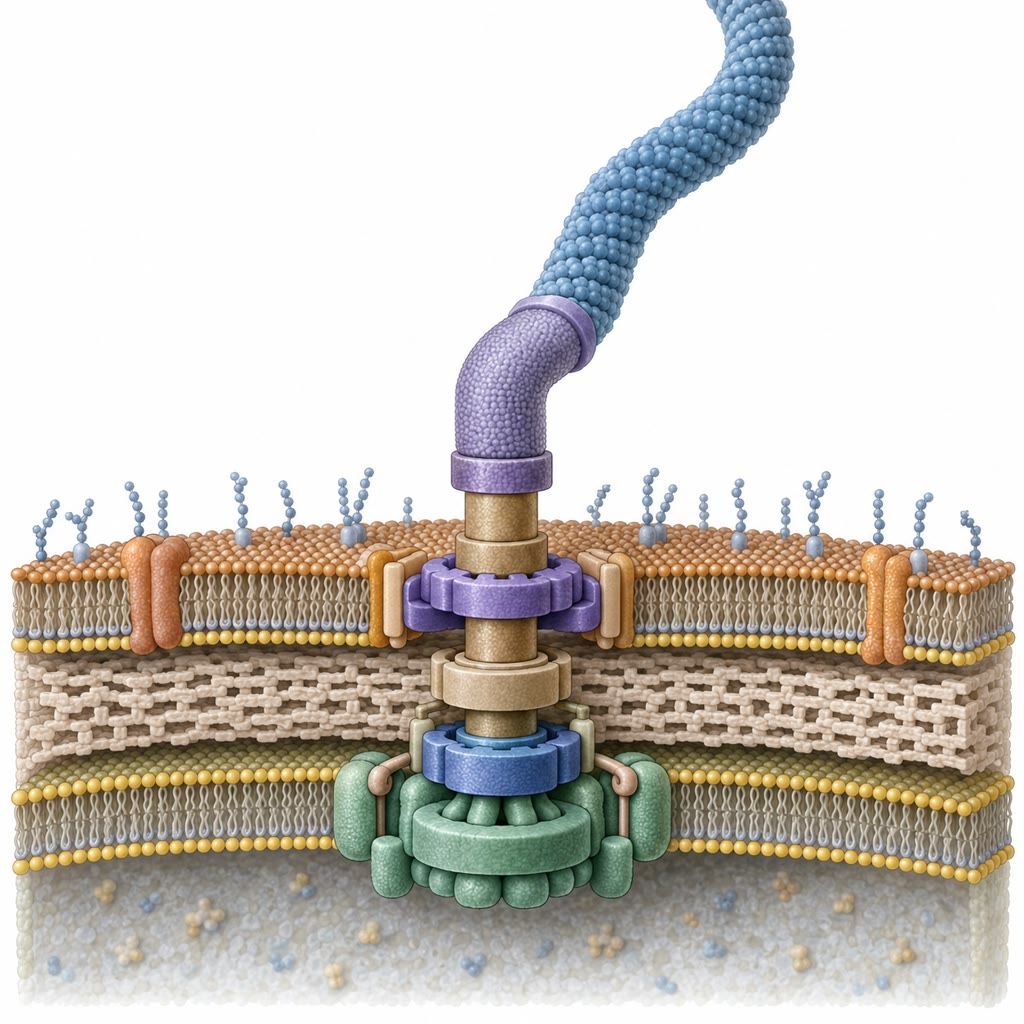
\includegraphics[width=0.36\linewidth]{images/book5/ai/b5-09-flagellar-motor.jpg}

{\small 左：气管的\omterm{def:b3:cytoskeleton-motility:cilia}{纤毛}上皮，扫描
电子显微镜下所见，\omterm{def:b3:cytoskeleton-motility:cilia}{纤毛}铺满圆顶状、分泌黏液的细胞之间。右：细菌
\omterm{prop:b3:cytoskeleton-motility:flagellar-motor}{鞭毛马达}，是细胞包膜中由环构成的旋转引擎，
由质子流驱动。}
\end{omfigure}

\begin{proposition}[细菌鞭毛马达]\label{prop:b3:cytoskeleton-motility:flagellar-motor}
\index{鞭毛马达}\index{直行与翻滚}
细菌鞭毛与真核鞭毛毫无关系：它是由鞭毛蛋白组成的刚性
螺旋丝，直径 \qty{20}{nm}，长达数微米，
由嵌入细胞包膜中的\emph{旋转马达}驱动——
转子由约 45 种蛋白质构成，外围环绕一圈定子单元，
每个定子单元都是一条通道，质子沿其梯度流入细胞，
每转一圈约有 1000 个质子通过。马达
最高转速可达 \qty{300}{Hz}，能在一毫秒内反转方向，
产生约 \qty{1000}{pN.nm} 的力矩；它由约 20 种蛋白质构成，
这些基因依次开启，开启顺序即部件的\omterm{def:b3:genomics:assembly}{组装}顺序，
由内向外。在\emph{E.~coli}中，
逆时针旋转使数根鞭毛聚成束，
形成螺旋桨，细胞\emph{直行}；转为顺时针旋转时，
鞭毛束散开，细胞\emph{翻滚}，并朝一个新的随机
方向前进。趋化通路调控的只是翻滚
的频率——条件改善时翻滚减少——而这已足以
使细胞沿梯度爬升。
\end{proposition}

\begin{remark}[细胞骨架是一个动词]\label{rem:b3:cytoskeleton-motility:verb}
本章所述几乎没有任何东西是骨骼那种意义上的结构：
\omterm{def:b3:cytoskeleton-motility:migration}{片状伪足}是一波聚合浪潮，
\cref{ch:b3:cell-cycle-apoptosis}中的纺锤体是一种
由生长与塌缩的\omterm{def:b3:cytoskeleton-motility:filaments}{微管}构成的稳态，\omterm{def:b3:cytoskeleton-motility:cilia}{纤毛}的摆动则是
马达的切换模式。更替并非细胞所能容忍的代价，而是
机制本身，这也是为何这些系统全都依赖核苷酸
水解运行，并在 ATP 耗尽后数分钟内停止，也是为何
能将聚合物冻结在任一状态的毒物——紫杉醇或
秋水仙碱、鬼笔环肽或细胞松弛素——同样致命。
\end{remark}

\section{练习}

\begin{exercise}[$\star$]\label{exo:b3:cytoskeleton-motility:1}
比较\omterm{def:b3:cytoskeleton-motility:filaments}{肌动蛋白丝}、\omterm{def:b3:cytoskeleton-motility:filaments}{微管}与\omterm{def:b3:cytoskeleton-motility:filaments}{中间纤维}在
直径、亚基、极性、核苷酸和典型功能方面的异同。
\end{exercise}

\begin{exercise}[$\star$]\label{exo:b3:cytoskeleton-motility:2}
定义\omterm{thm:b3:cytoskeleton-motility:treadmilling}{临界浓度}。为什么\omterm{def:b3:cytoskeleton-motility:filaments}{肌动蛋白丝}的两端
具有不同的\omterm{thm:b3:cytoskeleton-motility:treadmilling}{临界浓度}？
若两端的\omterm{thm:b3:cytoskeleton-motility:treadmilling}{临界浓度}相等，会发生什么？
\end{exercise}

\begin{exercise}[$\star$]\label{exo:b3:cytoskeleton-motility:3}
分别写出下列各过程所用的马达：沿\omterm{def:b3:cytoskeleton-motility:filaments}{微管}向细胞周边运输
囊泡；向细胞中心运输囊泡；应力纤维的收缩；
\omterm{def:b3:cytoskeleton-motility:cilia}{纤毛}的弯曲。并说明每种马达在其轨道上的运动方向。
\end{exercise}

\begin{exercise}[$\star$]\label{exo:b3:cytoskeleton-motility:4}
列出爬行循环的四个步骤，并说明前三个步骤各自由哪一种
Rho 家族 GTP 酶调控。
\end{exercise}

\begin{exercise}[$\star\star$]\label{exo:b3:cytoskeleton-motility:5}
某聚合物的正端有 $k_{\mathrm{on}} = \qty{5}{\micro M^{-1}.s^{-1}}$，
$k_{\mathrm{off}} = \qty{1}{s^{-1}}$；其负端 $k_{\mathrm{on}} =
\qty{1}{\micro M^{-1}.s^{-1}}$，$k_{\mathrm{off}} = \qty{0.8}{s^{-1}}$。
求两端的\omterm{thm:b3:cytoskeleton-motility:treadmilling}{临界浓度}与稳态浓度，
以及以每秒亚基数计的踏车速率；对于
\qty{2.7}{nm} 的亚基，求以纳米每秒计的踏车速率。
\end{exercise}

\begin{exercise}[$\star\star$]\label{exo:b3:cytoskeleton-motility:6}
\omterm{def:b3:cytoskeleton-motility:motors}{驱动蛋白}以 \qty{800}{nm/s} 的速度行走，步长 \qty{8}{nm}，
每步消耗一个 ATP。每个马达每秒消耗多少个 ATP？神经元的轴突长 \qty{1}{m}，
一次运输需要多长时间，一个马达在其间消耗多少个 ATP？
并将其与\cref{prop:b3:cytoskeleton-motility:physics}中的扩散时间进行比较。
\end{exercise}

\begin{exercise}[$\star\star$]\label{exo:b3:cytoskeleton-motility:7}
\omterm{def:b3:cytoskeleton-motility:motors}{肌球蛋白} V 每消耗一个 ATP 前进 \qty{36}{nm}。它的最大\omterm{prop:b3:cytoskeleton-motility:physics}{失速力}为多少，
以及为什么它比\omterm{def:b3:cytoskeleton-motility:motors}{驱动蛋白}的\omterm{prop:b3:cytoskeleton-motility:physics}{失速力}低？哪种马达更适合运载大负荷，
哪种更适合快速移动？
\end{exercise}

\begin{exercise}[$\star\star$]\label{exo:b3:cytoskeleton-motility:8}
预测下列药物对分裂细胞和爬行细胞的影响：(a)
紫杉醇，(b) 秋水仙碱，(c) 细胞松弛素，(d) Rac 抑制剂，并
根据作用机制分别加以解释。
\end{exercise}

\begin{exercise}[$\star\star$]\label{exo:b3:cytoskeleton-motility:9}
在\omterm{def:b3:cytoskeleton-motility:migration}{片状伪足}的 FRAP 实验中，荧光以
半衰期 \qty{20}{s} 恢复至初始值的 \qty{90}{\%}。求肌动蛋白
在网络中的停留时间及不动组分的比例？
斑点以 \qty{1.5}{\micro m/min} 的速度向后流动，而边缘
以 \qty{1}{\micro m/min} 的速度前进：肌动蛋白在
边缘处的聚合速率是多少？
\end{exercise}

\begin{exercise}[$\star\star\star$]\label{exo:b3:cytoskeleton-motility:10}
从 GTP 帽的角度解释\omterm{def:b3:cytoskeleton-motility:instability}{动态不稳定性}，并说明为何
维持在\omterm{thm:b3:cytoskeleton-motility:treadmilling}{临界浓度}略高处的\omterm{def:b3:cytoskeleton-motility:filaments}{微管}群体，
其长度呈双峰分布而非均匀分布。细胞从这种浪费 GTP 的行为
中获得了什么？
\end{exercise}

\begin{exercise}[$\star\star\star$]\label{exo:b3:cytoskeleton-motility:11}
直径为 \qty{2}{\micro m} 的细菌以 \qty{25}{\micro m/s} 的速度游动。在
这一尺度下的水中，黏性阻力占主导，马达一停转，细胞
便会在一纳米之内停下。试解释为什么往复运动（如划桨）
不能推动它，而旋转螺旋却可以，并估算
在 \qty{100}{Hz} 时马达每秒消耗的质子数。
\end{exercise}

\begin{exercise}[$\star\star\star$]\label{exo:b3:cytoskeleton-motility:12}
卡塔格纳综合征——\omterm{def:b3:cytoskeleton-motility:cilia}{纤毛}不动症——会导致慢性支气管炎、
男性不育，并且半数患者的心脏位于右侧。
试从\omterm{def:b3:cytoskeleton-motility:cilia}{轴丝}的生物学特性解释每一种表现，并说明为什么
最后一种表现只出现在半数患者中。
\end{exercise}

\section{问题：移动中的中性粒细胞}

\begin{problem}[{周末问题——中性粒细胞的肌动蛋白预算已清点，
踏车运动已算出，囊泡沿轴突运输的时间已与扩散时间比较，
马达效率已测定，爬行前沿的聚合与 ATP 消耗已算出，
最终求出踏车速率、穿过轴突所需的时间，以及
片状伪足每秒消耗的
ATP}]
\label{pb:b3:cytoskeleton-motility:1}
已知：中性粒细胞体积为 \qty{300}{\micro m^3}，肌动蛋白浓度为
\qty{200}{\micro M}，其中一半已聚合；每个亚基使丝延长 \qty{2.7}{nm}。
肌动蛋白速率常数
同\cref{ex:b3:cytoskeleton-motility:actin-numbers}。\omterm{def:b3:cytoskeleton-motility:motors}{驱动蛋白}：每步 \qty{8}{nm}，
速度 \qty{800}{nm/s}，\omterm{prop:b3:cytoskeleton-motility:physics}{失速力} \qty{6}{pN}；ATP 水解
$\Delta G = \qty{50}{kJ/mol}$；$k_{B}T = \qty{4.1}{pN.nm}$；囊泡
扩散系数 \qty{1}{\micro m^2/s}；轴突长 \qty{1}{m}。
\omterm{def:b3:cytoskeleton-motility:migration}{片状伪足}宽 \qty{20}{\micro m}，边缘每微米有
$200$ 根丝，以 \qty{10}{\micro m/min} 的速度前进；网络
在边缘后方 \qty{3}{\micro m} 处被解聚。

\medskip
\noindent\textbf{第一部分——肌动蛋白预算。}
\begin{enumerate}
  \item 细胞中共含多少个肌动蛋白分子，其中有
        多少个在丝中？
  \item 这些丝的总长度为多少？若平均每根丝长
        \qty{0.25}{\micro m}，共有多少根丝？
  \item 游离肌动蛋白浓度为 \qty{100}{\micro M}，远高于倒刺端的
        \omterm{thm:b3:cytoskeleton-motility:treadmilling}{临界浓度}。为什么丝不会简单地一直生长，
        直到单体耗尽？（涉及两种蛋白质。）
  \item 体外踏车运动：由速率常数计算 $C_{\text{ss}}$ 和 $J$，
        并求踏车速度，以纳米每秒计；
        再换算为微米每分钟。
  \item 细胞内的有效速度为 \qty{1}{\micro m/min}。调节因子使裸聚合物
        的速度提高了多少倍？
  \item 每个参与踏车运动的亚基消耗一个 ATP。若全部 $2\times 10^{5}$
        根丝以细胞内速度踏车运动，则每秒消耗多少个 ATP，
        这占细胞总周转量（约
        $10^{9}$ 个 ATP 每秒）的几分之几？
\end{enumerate}

\medskip
\noindent\textbf{第二部分——沿轴突运输的囊泡。}
\begin{enumerate}[resume]
  \item \omterm{def:b3:cytoskeleton-motility:motors}{驱动蛋白}驱动的囊泡沿轴突运输需要多长时间，
        马达蛋白需要走多少步、消耗多少个 ATP？
  \item 若仅靠扩散，穿过 \qty{1}{m} 需要多长时间？穿过
        \qty{10}{\micro m}（细胞体的宽度）需要多长时间？这一比较说明
        细胞在何种情形下可以
        依靠扩散？
  \item 分别以焦耳和 $k_{B}T$ 为单位，计算每个 ATP 的能量。
  \item 步长为 \qty{8}{nm} 的马达的最大力，
        以及\omterm{def:b3:cytoskeleton-motility:motors}{驱动蛋白}在失速状态下的效率。
  \item 半径为 \qty{100}{nm} 的囊泡，在黏度为
        \qty{0.01}{Pa.s}（水的十倍）的细胞质中以 \qty{800}{nm/s} 的速度运动，
        所受阻力为 $F = 6\pi\eta r v$。计算该阻力，并与\omterm{prop:b3:cytoskeleton-motility:physics}{失速力}比较：
        需要多少个马达？
  \item 神经元的轴突同时运载约 $10^{4}$ 个囊泡。该运输每秒
        消耗的 ATP 总量是多少，并与神经元放电每秒约
        $10^{9}$ 个 ATP 的开销相比如何？对于线粒体
        失效的神经元，
        这意味着什么？
\end{enumerate}

\medskip
\noindent\textbf{第三部分——前沿。}
\begin{enumerate}[resume]
  \item 将边缘推进速度换算为纳米每秒，并计算
        每根丝为跟上该速度，每秒必须添加的
        亚基数。
  \item 有多少根丝推动边缘，整个边缘每秒
        消耗多少个亚基？
  \item 每添加一个亚基即水解一个 ATP，之后再被回收。
        求突出所消耗的每秒 ATP 数，及其占细胞每秒 $10^{9}$
        个 ATP 的比例。
  \item 边缘后方的网络深 \qty{3}{\micro m}，并在此处解聚。
        亚基在网络中的寿命为多少，
        网络中任一时刻又有多少个亚基？
  \item 膜以约每根丝 \qty{1}{pN} 的力阻碍突出。计算每添加一个
        亚基所做的功（$F\times \qty{2.7}{nm}$），以 $k_{B}T$ 为
        单位表示，并判断布朗棘轮——一次热涨落
        打开 \qty{2.7}{nm} 的空位——
        是否合理。
  \item Listeria 的彗星尾为何不需要马达？若它招募同样的装置，
        其推进速度能有多快？
\end{enumerate}

\medskip
\noindent\textbf{第四部分——方向。}
\begin{enumerate}[resume]
  \item 中性粒细胞感受一种趋化因子，其浓度
        在其 \qty{10}{\micro m} 宽度上升高 \qty{2}{\%}。已知
        \num{50000} 个受体，且 $K_{d}$ 等于平均浓度，
        前半侧比后半侧多被占据的受体有多少个？
        （占据率 $\theta = C/(C +
        K_{d})$；每侧取受体数的一半。）
  \item 一侧被占据受体数的随机涨落约为该数的平方根。问题 19
        中的差异能否在单一时刻被探测到？
        在数秒内取平均，
        有何帮助？
  \item 为使细胞转向信号源，前沿与后部须分别激活
        哪一种小 GTP 酶？若细胞各处都持续激活
        Rac，会发生什么？
  \item 细胞从 \qty{30}{\micro m} 外、在 \qty{3}{min} 内
        抵达细菌。对照数据检验其速度。
  \item 缺乏 Arp2/3 复合体的细胞改以出泡运动移动，即由压力驱动的
        膜鼓泡取而代之。循环中哪一步被替代了，
        这说明肌动蛋白在其余各步中
        起什么作用？
  \item 整个爬行循环需时数分钟，而细胞在梯度改变时
        数秒内即可转向。试利用问题 16 中
        网络的寿命加以解释。
  \item 归纳：体外踏车运动的速度（问题 4）、
        囊泡沿轴突运输的时间（问题 7），以及
        突出所消耗的每秒 ATP 数（问题 15）。
\end{enumerate}
\end{problem}
